% ---------------------------------------------------------------------
%  CHƯƠNG 5 — CÀI ĐẶT VÀ THỬ NGHIỆM
% ---------------------------------------------------------------------
\chapter{Cài đặt và thử nghiệm}
\label{ch:caidat}

\begin{muctieu}
Chương này mô tả chi tiết môi trường phát triển, hiện thực hóa các mô-đun mã nguồn cốt lõi ở Backend và Frontend, trình bày thiết kế giao diện thực tế cùng các kịch bản kiểm thử toàn diện hệ thống.
\end{muctieu}

\section{Môi trường triển khai}

Hệ thống FoodAI được phát triển và kiểm thử trên môi trường phần cứng và phần mềm tiêu chuẩn:
\begin{itemize}[leftmargin=1.6em, itemsep=2pt]
  \item \textbf{Cấu hình phần cứng:} Bộ vi xử lý Intel Core i5/i7 thế hệ 11 trở lên, bộ nhớ trong RAM 16~GB, ổ cứng thể rắn SSD 512~GB.
  \item \textbf{Môi trường phần mềm:} Hệ điều hành Windows 11 64-bit / Ubuntu 22.04 LTS; môi trường thực thi Node.js v20.x, trình quản lý gói npm v10.x, cơ sở dữ liệu MySQL 8.0.
  \item \textbf{Cấu hình biến môi trường (\code{.env}):} Quản lý các tham số nhạy cảm gồm \code{GEMINI\_API\_KEY}, \code{PEXELS\_API\_KEY}, \code{JWT\_SECRET}, \code{PORT=5000} và thông tin kết nối cơ sở dữ liệu.
\end{itemize}

\section{Cài đặt các thành phần cốt lõi phía Backend}

\subsection{Mô-đun dịch vụ Gemini AI và Trích xuất JSON kiên cố}

Mô-đun \code{gemini.service.ts} đảm nhận việc kết nối tới Google Generative AI, gửi prompt có cấu trúc và phân tích cú pháp JSON trả về. Mã nguồn~\ref{lst:gemini_service} minh họa cơ chế gọi mô hình và làm sạch chuỗi phản hồi.

\begin{lstlisting}[language=Java, caption={Khởi tạo Google Gemini AI và xử lý JSON an toàn.}, label={lst:gemini_service}]
import { GoogleGenerativeAI } from '@google/generative-ai';

// Initialize Gemini Generative AI client
const genAI = new GoogleGenerativeAI(process.env.GEMINI_API_KEY || '');

export async function suggestWithGemini(ingredients: string[], userId: string, count: number = 6) {
  const model = genAI.getGenerativeModel({
    model: 'gemini-3.6-flash',
    generationConfig: {
      responseMimeType: 'application/json',
      temperature: 0.6,
    },
  });

  const prompt = buildChefPrompt(ingredients, count);
  const result = await model.generateContent(prompt);
  const rawText = result.response.text();

  // Clean markdown code fence if present
  let cleanJson = rawText.trim()
    .replace(/^```json\s*/, '')
    .replace(/\s*```$/, '');

  // Parse and validate JSON structure safely
  const parsed = JSON.parse(cleanJson);
  const recipes = Array.isArray(parsed) ? parsed : (parsed?.recipes || []);
  
  return sanitizeAndDeduplicate(recipes);
}
\end{lstlisting}

\noindent\textbf{Mô tả:} Mã nguồn~\ref{lst:gemini_service} mô tả hàm \code{suggestWithGemini} trong dịch vụ \code{gemini.service.ts}, bao gồm các bước: khởi tạo client GoogleGenerativeAI, cấu hình model \code{gemini-3.6-flash} với định dạng phản hồi bắt buộc là JSON, gửi prompt phân vai chuyên gia ẩm thực, làm sạch chuỗi phản hồi (loại bỏ markdown fence) và phân tích cú pháp an toàn với cơ chế khử trùng lặp.

\noindent\textbf{Diễn giải:} Đoạn mã thể hiện giải pháp kỹ thuật kiên cố để khắc phục tính bất định của LLM. Việc thiết lập \code{responseMimeType: 'application/json'} kết hợp bộ lọc Regex làm sạch mã Markdown đảm bảo hệ thống không bị lỗi cú pháp \code{JSON.parse()} ngay cả khi mô hình tự ý bọc khối văn bản trong ký hiệu code fence. Nhiệt độ (temperature) được tinh chỉnh ở mức 0.6 là điểm cân bằng tối ưu giữa việc sáng tạo công thức ẩm thực mới lạ và việc tuân thủ các quy tắc dinh dưỡng khắt khe.

\subsection{Mô-đun chuẩn hóa NLP tiếng Việt và So khớp nguyên liệu}

Mã nguồn~\ref{lst:vietnamese_nlp} minh họa hàm loại bỏ dấu thanh Unicode NFD và thuật toán kiểm tra ranh giới từ nguyên vẹn \code{containsWord}, giúp triệt tiêu các lỗi nhầm lẫn nghiêm trọng trong tiếng Việt.

\begin{lstlisting}[language=Java, caption={Chuẩn hóa tiếng Việt và kiểm tra ranh giới từ nguyên vẹn.}, label={lst:vietnamese_nlp}]
// Remove Vietnamese diacritics via NFD decomposition
export function removeVietnameseAccents(str: string): string {
  return str
    .normalize('NFD')
    .replace(/[\u0300-\u036f]/g, '')
    .replace(/d/g, 'd')
    .replace(/D/g, 'D')
    .toLowerCase()
    .trim();
}

// Check whole-word boundary with negative semantic exclusions
export function containsWord(fullText: string, targetWord: string): boolean {
  const f = removeVietnameseAccents(fullText);
  const t = removeVietnameseAccents(targetWord);
  if (!f || !t) return false;

  // Handle specific Vietnamese food ambiguities
  if (t === 'ca' && (f.includes('ca chua') || f.includes('ca tim') || f.includes('ca rot'))) {
    return false; // Tomato/Eggplant/Carrot is NOT fish
  }
  if (t === 'bo' && (f.includes('bo toi') || f.includes('qua bo') || f.includes('bo lat'))) {
    return false; // Butter/Avocado is NOT beef
  }
  if (t === 'ga' && (f.includes('dau ga') || f.includes('nam dui ga'))) {
    return false; // Chickpea/Mushroom is NOT chicken
  }

  // Exact word boundary regex check
  const escaped = t.replace(/[.*+?^${}()|[\]\\]/g, '\\$&');
  const regex = new RegExp(`(^|[^a-z0-9])${escaped}([^a-z0-9]|$)`, 'i');
  return regex.test(f);
}
\end{lstlisting}

\noindent\textbf{Mô tả:} Mã nguồn~\ref{lst:vietnamese_nlp} trình bày hai hàm tiền xử lý ngôn ngữ tự nhiên tiếng Việt: hàm \code{removeVietnameseAccents} chuyển đổi chuỗi có dấu thành không dấu bằng phân rã chuẩn Unicode NFD, và hàm \code{containsWord} kiểm tra sự tồn tại của từ đích dựa trên ranh giới từ nguyên vẹn kết hợp các luật loại trừ ngữ nghĩa phủ định.

\noindent\textbf{Diễn giải:} Đây là lớp bảo vệ then chốt loại bỏ triệt để các lỗi nhận diện sai lầm kinh điển của NLP tiếng Việt. Nhờ có các điều kiện ngoại lệ phủ định, hệ thống không bao giờ hiểu nhầm ``cà chua'', ``cà tím'' là nguyên liệu ``cá''; không nhận nhầm ``bơ tỏi'', ``bơ lạt'' là ``thịt bò''; và không nhầm ``nấm đùi gà'', ``đậu gà'' là ``thịt gà''. Biểu thức chính quy kiểm tra ranh giới từ nguyên vẹn ngăn chặn hiện tượng khớp chuỗi con vô nghĩa, làm nền tảng cho thuật toán kiểm soát ràng buộc hoạt động chuẩn xác 100\%.

\subsection{Mô-đun trích xuất đạm chính và Chấm điểm ảnh Cookpad}

Mã nguồn~\ref{lst:image_service} minh họa thuật toán trích xuất thành phần đạm chính \code{extractPrimaryIngredients} và loại bỏ ảnh tiêu cực (cơm bento tạo hình, cơm ăn dặm trẻ em).

\begin{lstlisting}[language=Java, caption={Trích xuất nhóm đạm chính và chấm điểm ảnh món ăn.}, label={lst:image_service}]
export function extractPrimaryIngredients(text: string): Set<string> {
  const norm = removeVietnameseAccents(text);
  const detected = new Set<string>();

  if (/\b(ga|uc\s+ga|canh\s+ga|dui\s+ga)\b/.test(norm)) detected.add('ga');
  if (/\b(bo|thit\s+bo|bap\s+bo|nam\s+bo)\b/.test(norm)) detected.add('bo');
  if (/\b(heo|lon|ba\s+chi|thit\s+bam|suon)\b/.test(norm)) detected.add('heo');
  if (/\b(tom|tep|tom\s+su)\b/.test(norm)) detected.add('tom');
  if (/\b(ca|ca\s+loc|ca\s+thu|ca\s+hoi)\b/.test(norm)) detected.add('ca');

  return detected;
}

export function scoreRecipeCard(cardTitle: string, targetDish: string): number {
  const normTitle = removeVietnameseAccents(cardTitle);
  // Exclude unwanted child bento and baby food
  const hardNegatives = ['bento', 'an dam', 'be', 'mam com', 'combo'];
  for (const neg of hardNegatives) {
    if (normTitle.includes(neg)) return -100;
  }
  return calculateKeywordCoverage(cardTitle, targetDish);
}
\end{lstlisting}

\noindent\textbf{Mô tả:} Mã nguồn~\ref{lst:image_service} thể hiện hai hàm quan trọng trong mô-đun \code{image.service.ts}: hàm \code{extractPrimaryIngredients} trích xuất tập hợp các nhóm đạm động vật chủ đạo (gà, bò, heo, tôm, cá) từ văn bản công thức, và hàm \code{scoreRecipeCard} chấm điểm tương đồng từ khóa của thẻ ảnh Cookpad đồng thời áp dụng điểm phạt tuyệt đối cho các từ khóa ảnh tiêu cực.

\noindent\textbf{Diễn giải:} Hàm trích xuất đạm đảm bảo nguyên tắc nhất quán giữa hình ảnh và nội dung công thức: nếu món ăn là món cá, ảnh gán vào bắt buộc phải là ảnh món cá thực tế. Thuật toán chấm điểm thẻ ảnh loại trừ triệt để các hình ảnh cơm hộp bento hoạt hình, thức ăn dặm cho trẻ nhỏ hoặc mâm cơm combo nhiều món (điểm phạt $-100$), đảm bảo các bức ảnh được gán vào món ăn luôn mang tính thẩm mỹ cao, chân thực và phù hợp với món ăn gia đình Việt Nam.

\section{Cài đặt phía Frontend và Giao diện người dùng}

Ứng dụng Frontend của hệ thống FoodAI được xây dựng dựa trên nền tảng React 18, Vite và TailwindCSS, tối ưu hóa giao diện người dùng theo phong cách hiện đại, trực quan và đáp ứng linh hoạt trên nhiều kích thước màn hình. Các giao diện thực tế của hệ thống được chia thành hai phân hệ độc lập: phân hệ Khách hàng (Client Web Application) và phân hệ Quản trị viên (Admin Panel).

\subsection{Giao diện phân hệ Khách hàng (Client Web Application)}

Phân hệ khách hàng cung cấp các tính năng hỗ trợ người dùng từ khâu xác thực, nhập liệu nguyên liệu, nhận kết quả gợi ý ẩm thực từ AI Chef cho đến lưu trữ và quản lý công thức yêu thích.

\begin{figure}[H]
\centering
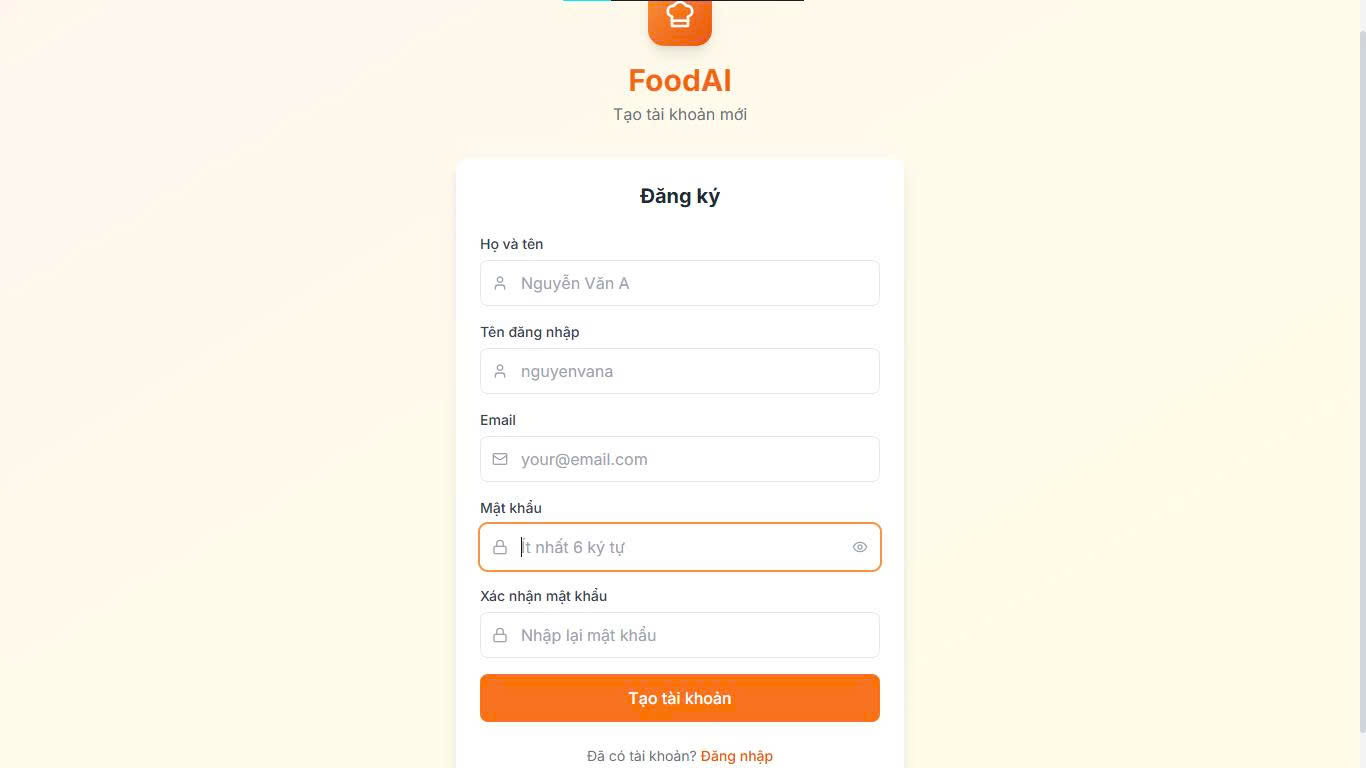
\includegraphics[width=0.88\textwidth]{figs/ui_dang_ky.jpg}
\caption{Giao diện Đăng ký tài khoản người dùng mới trên FoodAI.}
\label{fig:ui_dang_ky}
\end{figure}

\noindent\textbf{Mô tả:} Hình~\ref{fig:ui_dang_ky} hiển thị giao diện Đăng ký tài khoản người dùng mới, bao gồm form nhập liệu 5 trường: Họ và tên, Tên đăng nhập, Email, Mật khẩu và Xác nhận mật khẩu, cùng nút hành động ``Đăng ký ngay'' và liên kết chuyển nhanh đến trang Đăng nhập.

\noindent\textbf{Diễn giải:} Giao diện được thiết kế tối giản, tập trung vào trải nghiệm người dùng với các thông báo lỗi trực quan (validation inline). Việc xác thực dữ liệu ngay tại Client giúp người dùng kịp thời sửa sai khi nhập email không đúng định dạng hoặc mật khẩu chưa đủ 6 ký tự. Khi người dùng gửi biểu mẫu, mật khẩu được mã hóa an toàn bằng BCrypt trước khi ghi vào cơ sở dữ liệu MySQL, bảo đảm an toàn thông tin cá nhân.

\begin{figure}[H]
\centering
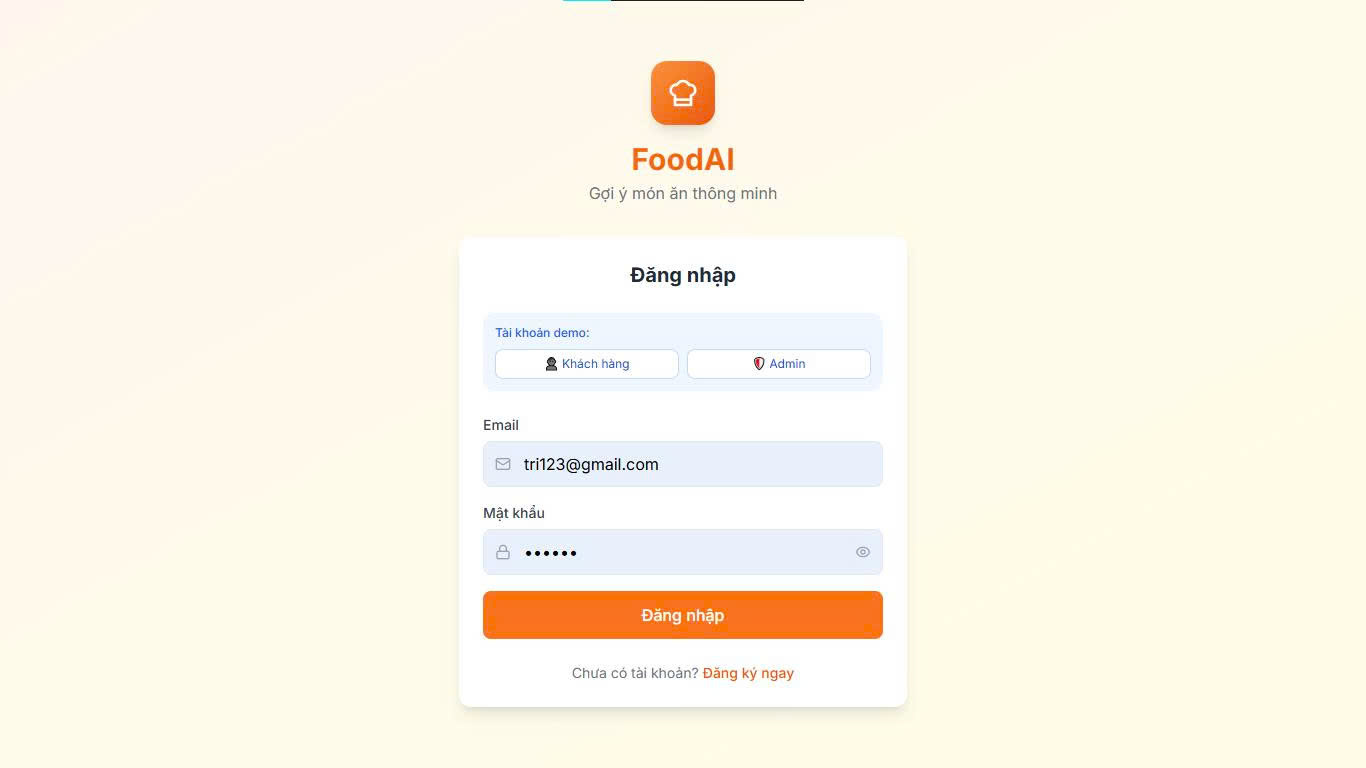
\includegraphics[width=0.88\textwidth]{figs/ui_dang_nhap.jpg}
\caption{Giao diện Đăng nhập hệ thống (hỗ trợ phím tắt tài khoản Demo).}
\label{fig:ui_dang_nhap}
\end{figure}

\noindent\textbf{Mô tả:} Hình~\ref{fig:ui_dang_nhap} thể hiện giao diện Đăng nhập hệ thống gồm form xác thực Email và Mật khẩu, cùng hai nút tiện ích chọn nhanh tài khoản thử nghiệm: Khách hàng (tri123@gmail.com) và Quản trị viên (admin@foodsystem.com).

\noindent\textbf{Diễn giải:} Thiết kế giao diện tích hợp hai nút Demo giúp hội đồng đánh giá và người dùng trải nghiệm ngay lập tức các luồng nghiệp vụ mà không mất thời gian đăng ký mới. Sau khi đăng nhập thành công, hệ thống cấp phát mã JWT token lưu vào localStorage và tự động điều hướng: người dùng thông thường vào Dashboard trang chủ, còn tài khoản Admin được chuyển thẳng đến bảng điều khiển quản trị.

\begin{figure}[H]
\centering
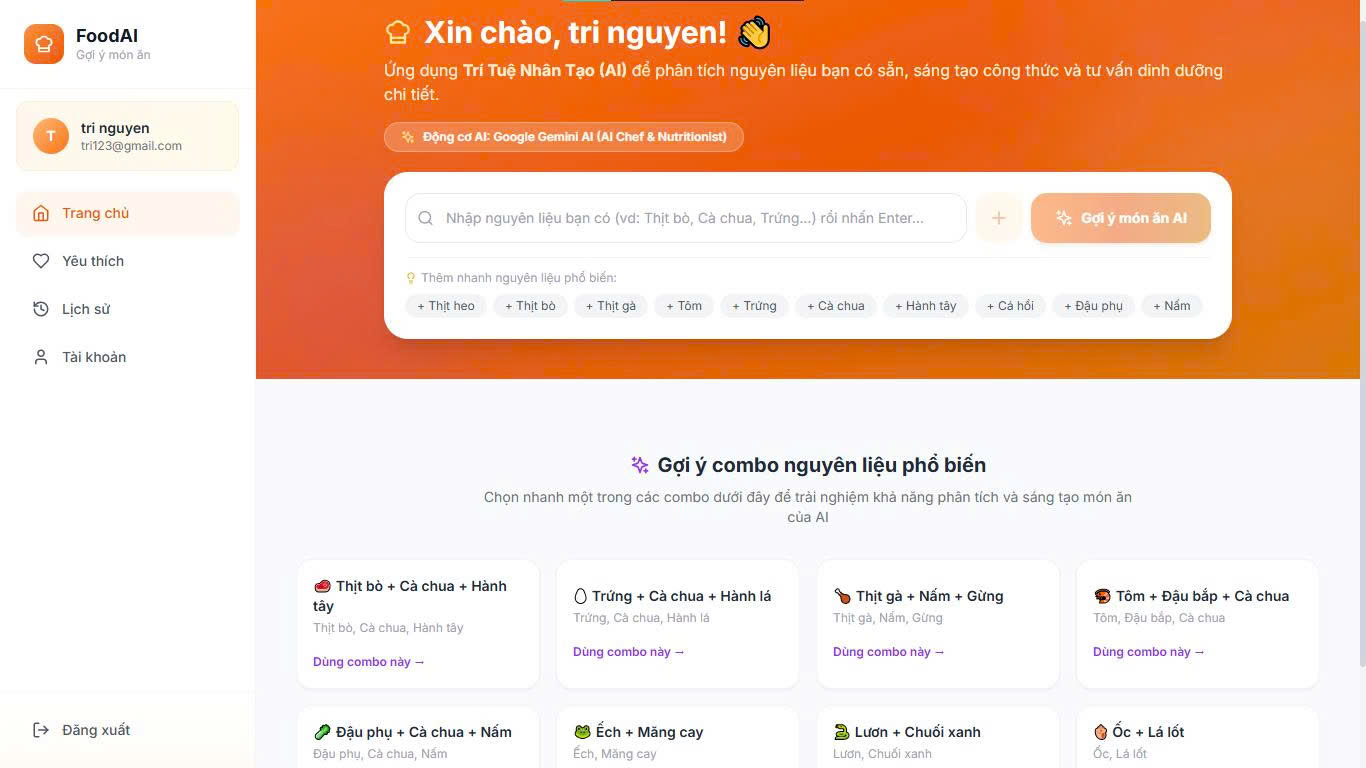
\includegraphics[width=0.96\textwidth]{figs/ui_trang_chu_dashboard.jpg}
\caption{Giao diện Bảng điều khiển Gợi ý món ăn thông minh (Home Dashboard).}
\label{fig:ui_dashboard}
\end{figure}

\noindent\textbf{Mô tả:} Hình~\ref{fig:ui_dashboard} thể hiện giao diện Bảng điều khiển trang chủ (Home Dashboard) --- phân hệ tương tác cốt lõi của người dùng, gồm thanh nhập nguyên liệu động dạng tag màu, danh sách nút chọn nhanh nguyên liệu phổ biến, bộ sưu tập combo món ăn mẫu và nút kích hoạt ``Gợi ý món ăn AI''.

\noindent\textbf{Diễn giải:} Đây là trung tâm trải nghiệm của hệ thống FoodAI. Người dùng có thể linh hoạt nhập nguyên liệu bằng cách gõ phím hoặc nhấn 1-click vào các nguyên liệu thông dụng có sẵn. Bố cục trực quan giúp giảm tối đa thao tác nhập liệu rườm rà. Khi nhấn nút gợi ý, hệ thống gửi yêu cầu lên Backend để phối hợp giữa mô hình Gemini AI và kho ảnh Cookpad, trả về kết quả gợi ý chỉ sau vài giây.

\begin{figure}[H]
\centering
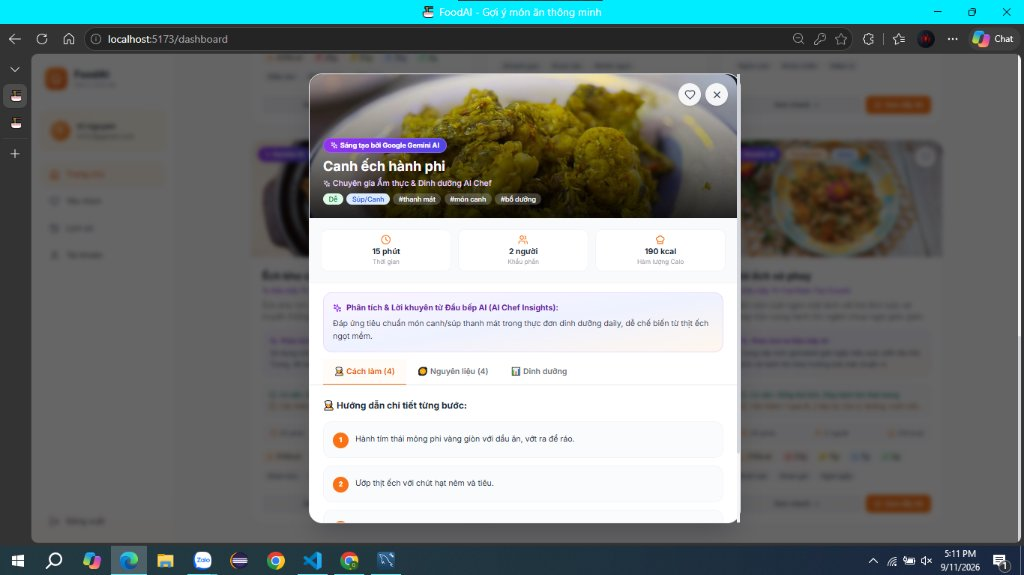
\includegraphics[width=0.82\textwidth]{figs/ui_modal_chi_tiet_mon.jpg}
\caption{Giao diện Modal Chi tiết Công thức nấu và Phân tích dinh dưỡng từ AI Chef.}
\label{fig:ui_modal_detail}
\end{figure}

\noindent\textbf{Mô tả:} Hình~\ref{fig:ui_modal_detail} hiển thị cửa sổ Modal chi tiết món ăn khi người dùng nhấn xem công thức, cấu trúc thành 3 tab chức năng: Tab Cách làm (hướng dẫn nấu từng bước), Tab Nguyên liệu (định lượng chuẩn và đánh dấu nguyên liệu có sẵn), và Tab Dinh dưỡng (bảng 8 chỉ số vi chất kèm lời khuyên chuyên gia AI Chef).

\noindent\textbf{Diễn giải:} Modal này minh chứng cho giá trị chuyên sâu của hệ thống so với các website dạy nấu ăn thông thường. Lời khuyên ẩm thực từ AI Chef cung cấp bí quyết canh lửa và tẩm ướp chuẩn vị, trong khi bảng chỉ số dinh dưỡng giúp người nội trợ dễ dàng cân đối năng lượng và vi chất cho bữa cơm gia đình. Thiết kế dạng tab giúp phân tách luồng thông tin rõ ràng, không gây rối mắt cho người dùng.

\begin{figure}[H]
\centering
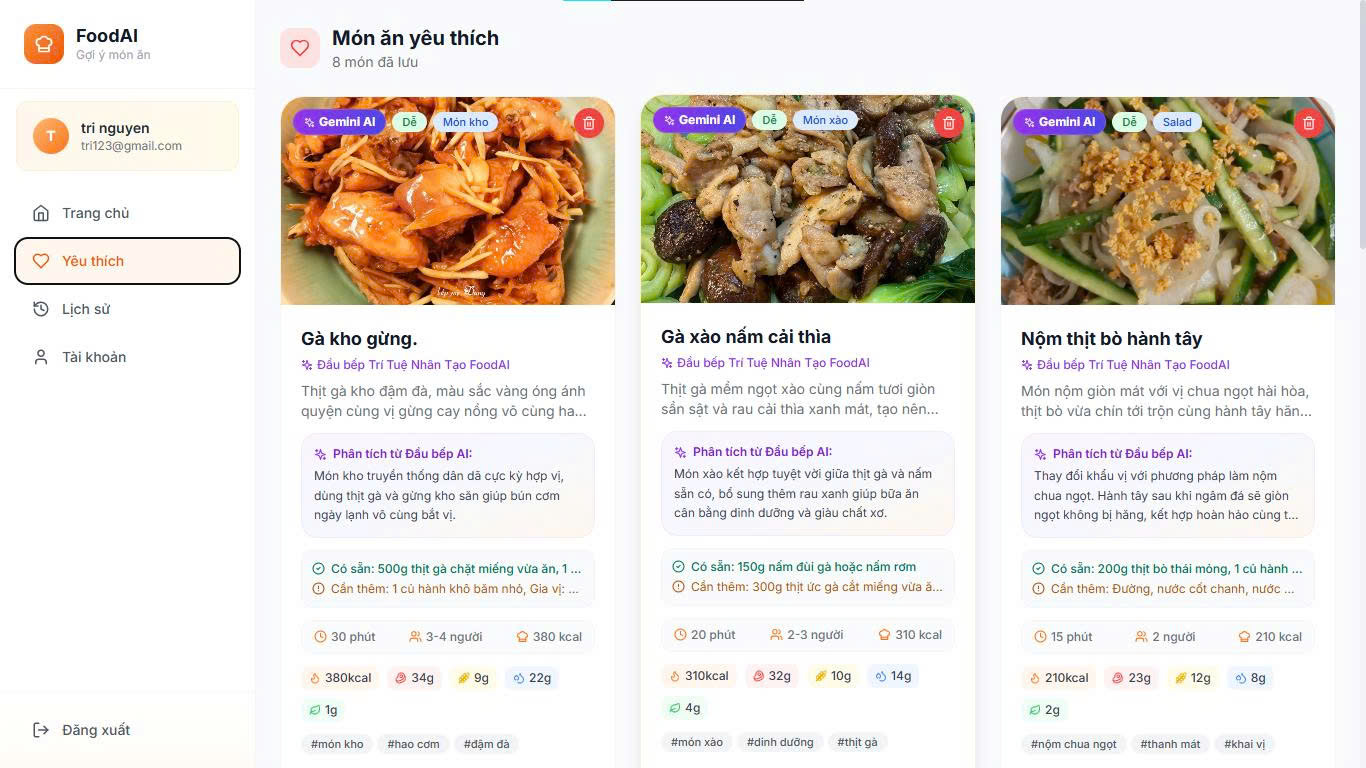
\includegraphics[width=0.96\textwidth]{figs/ui_mon_an_yeu_thich.jpg}
\caption{Giao diện Quản lý Danh sách Món ăn yêu thích của người dùng.}
\label{fig:ui_favorites}
\end{figure}

\noindent\textbf{Mô tả:} Hình~\ref{fig:ui_favorites} mô tả trang quản lý danh sách món ăn yêu thích, hiển thị bộ sưu tập các món ăn mà người dùng đã bấm lưu (icon trái tim) dưới dạng lưới thẻ Recipe Card trực quan.

\noindent\textbf{Diễn giải:} Tính năng này đóng vai trò như một cuốn sổ tay nấu ăn cá nhân hóa trực tuyến. Mỗi thẻ món ăn hiển thị đầy đủ hình ảnh, thời gian nấu, khẩu phần, mức calo và nút xóa khỏi bộ sưu tập. Dữ liệu được liên kết chặt chẽ với userId trong CSDL MySQL, đảm bảo tính riêng tư và cho phép người dùng dễ dàng xem lại công thức để chế biến vào các ngày tiếp theo mà không cần phải tìm kiếm lại từ đầu.

\begin{figure}[H]
\centering
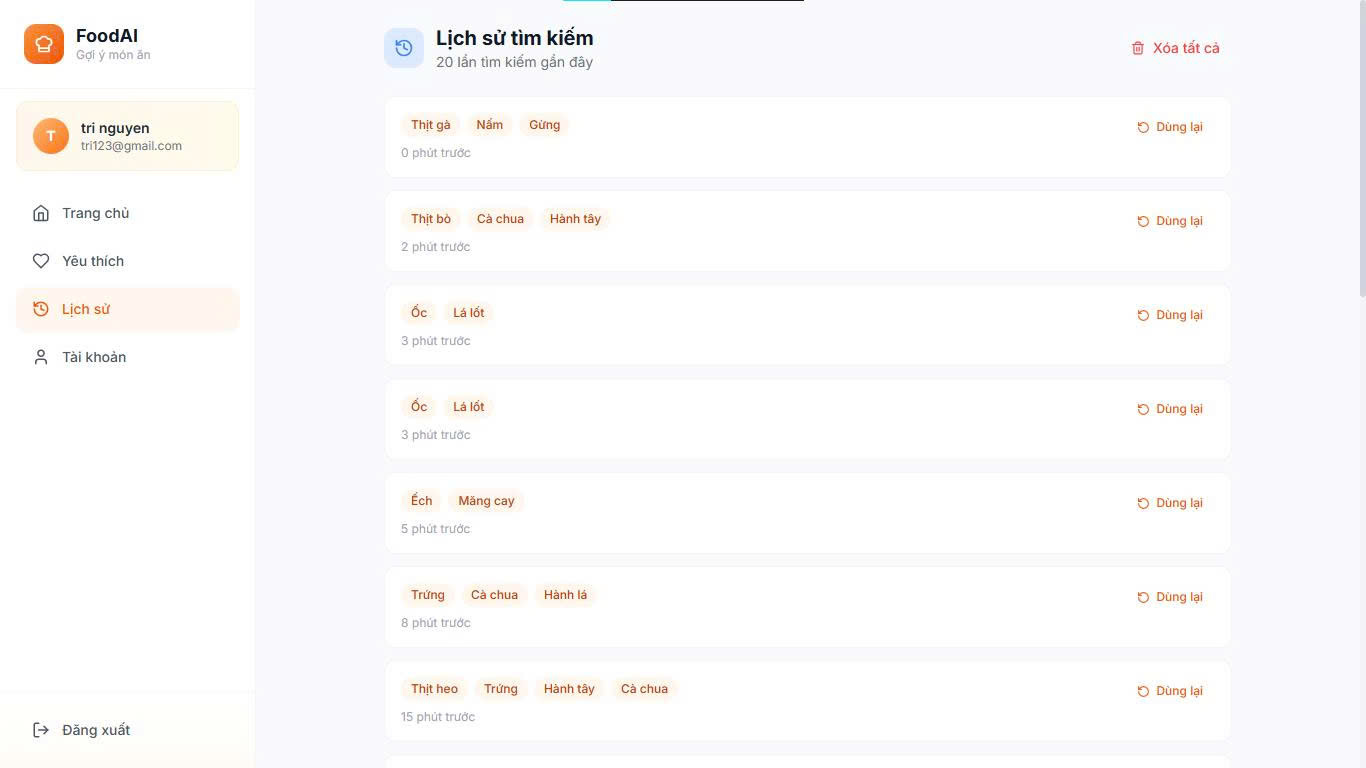
\includegraphics[width=0.96\textwidth]{figs/ui_lich_su_tim_kiem.jpg}
\caption{Giao diện Lịch sử tìm kiếm nguyên liệu và Tính năng tái sử dụng (Dùng lại).}
\label{fig:ui_history}
\end{figure}

\noindent\textbf{Mô tả:} Hình~\ref{fig:ui_history} thể hiện trang Lịch sử tìm kiếm nguyên liệu, liệt kê danh sách tối đa 20 phiên tìm kiếm gần nhất theo thứ tự thời gian, mỗi phiên hiển thị các thẻ tag nguyên liệu đã nhập và nút bấm ``Dùng lại''.

\noindent\textbf{Diễn giải:} Chức năng này giải quyết nhu cầu thực tế của người dùng khi thường xuyên lặp lại các bữa cơm gia đình với những nguyên liệu quen thuộc. Bằng cách nhấn nút ``Dùng lại'', toàn bộ tập nguyên liệu của phiên tìm kiếm trước đó sẽ được tự động điền ngược lại vào thanh tìm kiếm trên trang chủ chỉ với 1 cú nhấp chuột, giúp tiết kiệm thời gian và nâng cao đáng kể sự tiện dụng của ứng dụng.

\begin{figure}[H]
\centering
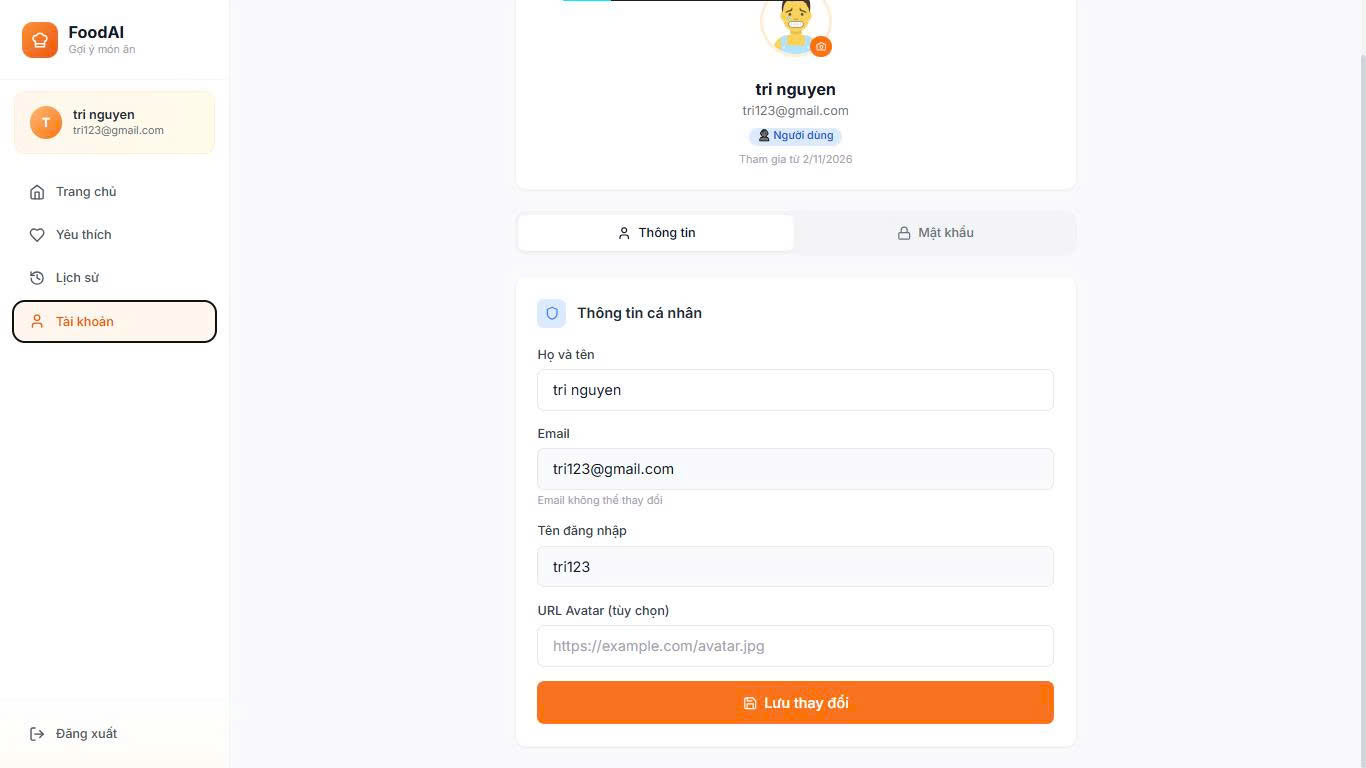
\includegraphics[width=0.96\textwidth]{figs/ui_thong_tin_tai_khoan.jpg}
\caption{Giao diện Quản lý Thông tin tài khoản cá nhân và Đổi mật khẩu.}
\label{fig:ui_profile}
\end{figure}

\noindent\textbf{Mô tả:} Hình~\ref{fig:ui_profile} thể hiện giao diện trang Cá nhân của người dùng, chia làm hai phân vùng: Thông tin tài khoản (ảnh đại diện Avatar, họ tên, email, ngày tham gia) và Biểu mẫu Đổi mật khẩu an toàn.

\noindent\textbf{Diễn giải:} Giao diện cung cấp cho người dùng quyền tự quản lý hồ sơ cá nhân và tăng cường bảo mật tài khoản. Cơ chế đổi mật khẩu bắt buộc phải nhập chính xác mật khẩu hiện tại trước khi thiết lập mật khẩu mới, ngăn ngừa nguy cơ tài khoản bị chiếm quyền khi người dùng vô tình để lộ phiên làm việc trên các thiết bị công cộng.

\subsection{Giao diện phân hệ Quản trị viên (Admin Panel)}

Phân hệ Quản trị viên dành riêng cho vai trò Admin (\code{role = 'admin'}), cung cấp bảng điều khiển toàn diện phục vụ quản trị dữ liệu, giám sát mô hình Trí tuệ Nhân tạo và theo dõi tài nguyên hệ thống.

\begin{figure}[H]
\centering
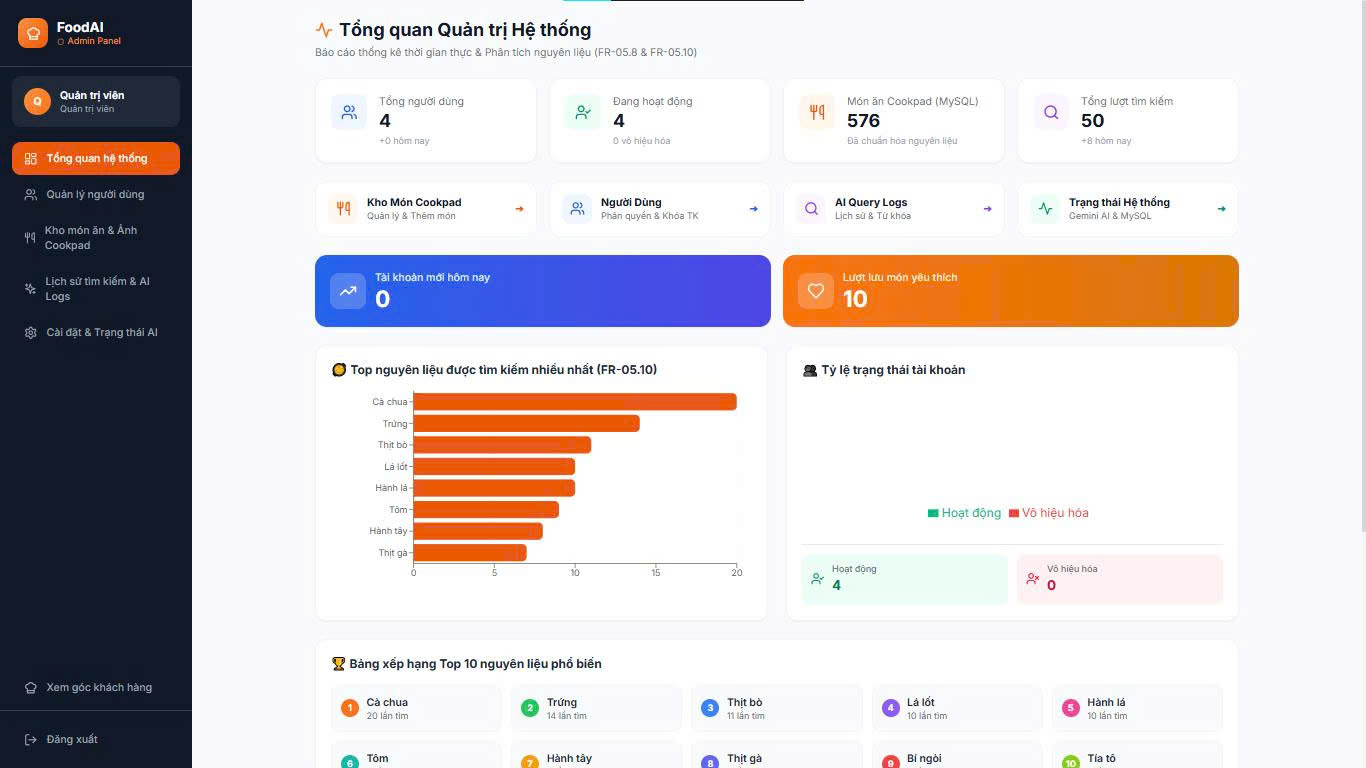
\includegraphics[width=0.96\textwidth]{figs/ui_admin_tong_quan.jpg}
\caption{Giao diện Bảng điều khiển Tổng quan Quản trị và Thống kê thời gian thực.}
\label{fig:ui_admin_overview}
\end{figure}

\noindent\textbf{Mô tả:} Hình~\ref{fig:ui_admin_overview} thể hiện trang Tổng quan Quản trị (Admin Overview), bao gồm hệ thống các thẻ đo lường KPI (Tổng người dùng, tài khoản hoạt động, quy mô kho món ăn, tổng lượt tìm kiếm) và biểu đồ cột thống kê Top 10 nguyên liệu được tìm kiếm nhiều nhất.

\noindent\textbf{Diễn giải:} Trang tổng quan cung cấp cho quản trị viên cái nhìn toàn diện về hoạt động của hệ thống theo thời gian thực. Biểu đồ Top 10 nguyên liệu phổ biến (Cà chua, Trứng, Thịt bò, Tôm...) giúp quản trị viên phân tích xu hướng ẩm thực của người dùng, từ đó định hướng mở rộng kho công thức và bổ sung hình ảnh Cookpad cho các nhóm nguyên liệu được quan tâm nhiều nhất.

\begin{figure}[H]
\centering
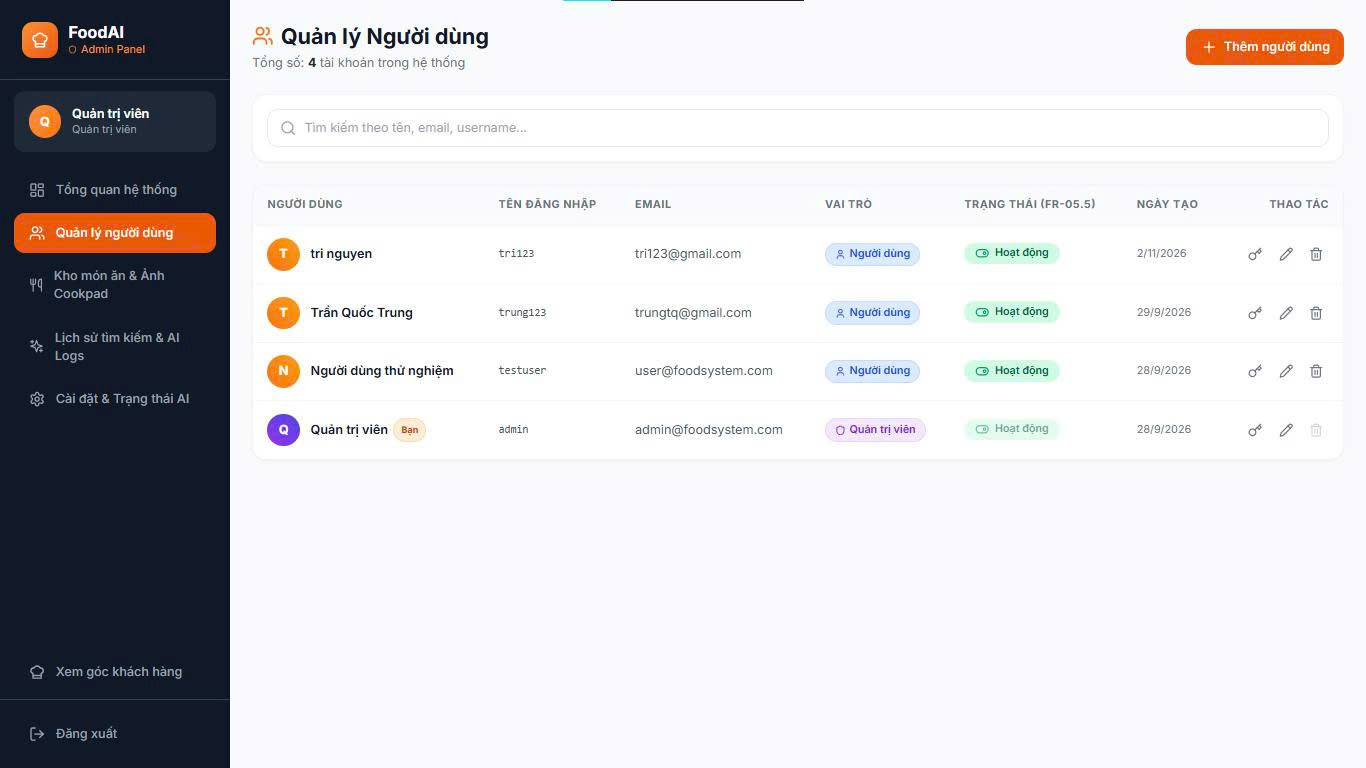
\includegraphics[width=0.96\textwidth]{figs/ui_admin_quan_ly_nguoi_dung.jpg}
\caption{Giao diện Quản lý danh sách Người dùng và Phân quyền tài khoản.}
\label{fig:ui_admin_users}
\end{figure}

\noindent\textbf{Mô tả:} Hình~\ref{fig:ui_admin_users} mô tả bảng dữ liệu quản lý người dùng với các cột thông tin: Avatar, Họ tên, Email, Vai trò (Admin/User), Trạng thái (Hoạt động/Bị khóa) và các nút thao tác chỉnh sửa, đổi mật khẩu và kích hoạt/khóa tài khoản.

\noindent\textbf{Diễn giải:} Phân hệ này cho phép Admin quản trị toàn bộ người dùng trong hệ thống với tính năng tìm kiếm thời gian thực và phân trang thông minh. Đặc biệt, hệ thống tích hợp chốt an toàn ở cả Frontend và Backend ngăn chặn Quản trị viên tự khóa tài khoản của chính mình, đảm bảo hệ thống luôn luôn có quyền điều hành khả dụng.

\begin{figure}[H]
\centering
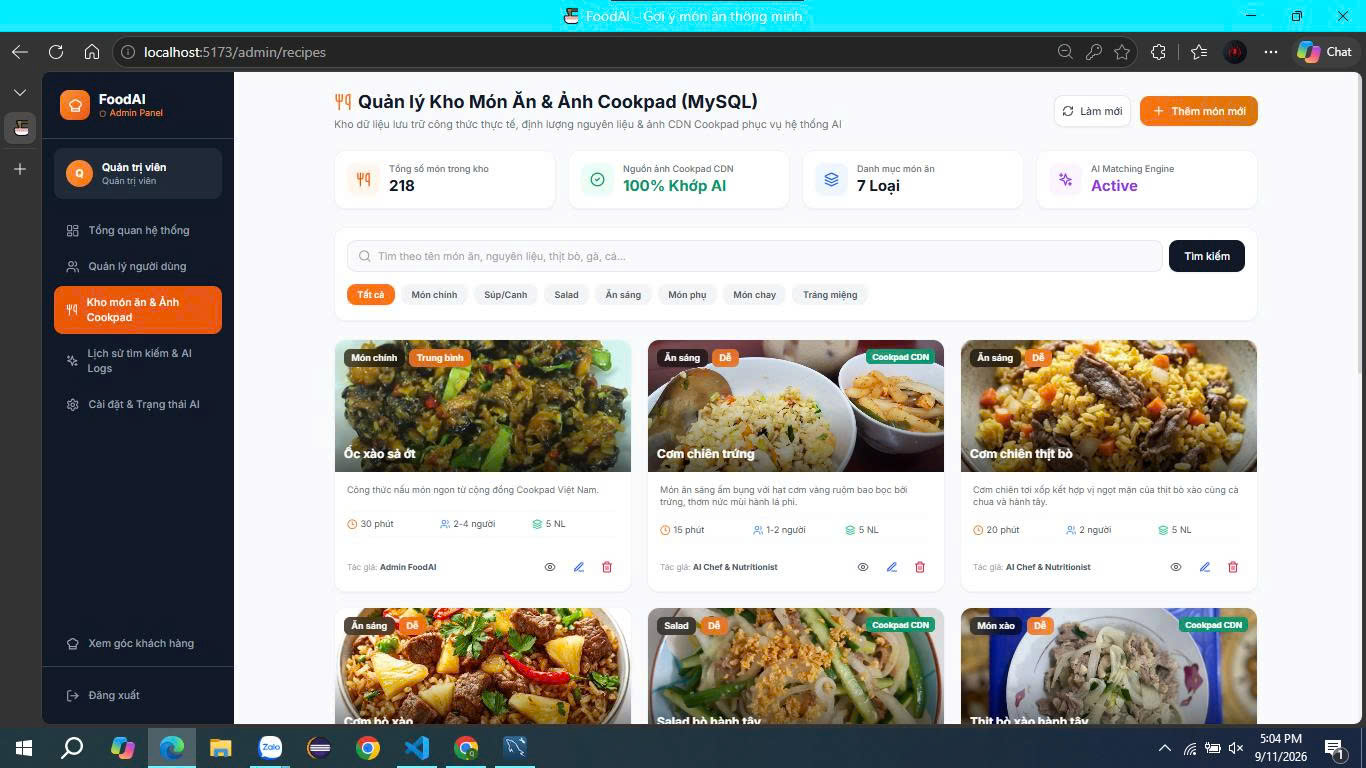
\includegraphics[width=0.96\textwidth]{figs/ui_admin_kho_mon_an.jpg}
\caption{Giao diện Quản lý Kho Món Ăn và Hình ảnh Cookpad CDN (MySQL).}
\label{fig:ui_admin_recipes}
\end{figure}

\noindent\textbf{Mô tả:} Hình~\ref{fig:ui_admin_recipes} mô tả giao diện Quản lý Kho Món Ăn Cookpad trong CSDL MySQL, gồm thanh tìm kiếm món ăn, bộ lọc theo 7 danh mục ẩm thực, và lưới hiển thị các thẻ món ăn kèm hình ảnh CDN thực tế, độ khó, thời gian nấu và thông tin tác giả.

\noindent\textbf{Diễn giải:} Đây là trung tâm quản trị cơ sở tri thức ẩm thực nội bộ với hơn 550 món ăn Việt Nam đã được chuẩn hóa. Nhờ kho dữ liệu này, hệ thống vừa có thể cung cấp kho ảnh chất lượng cao để gán vào các món ăn do AI tạo sinh, vừa đóng vai trò làm nguồn dữ liệu dự phòng (Fallback) khi xảy ra sự cố gián đoạn kết nối tới máy chủ Google Gemini.

\begin{figure}[H]
\centering
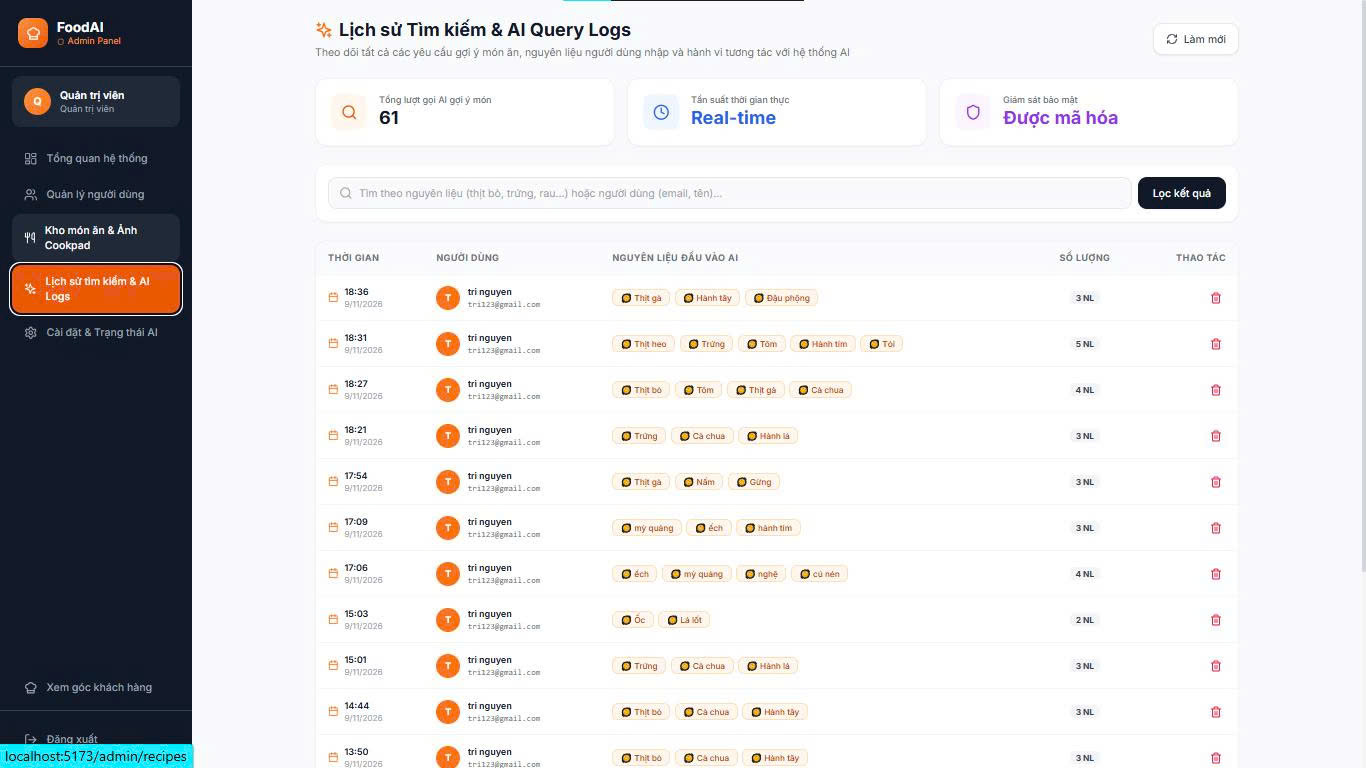
\includegraphics[width=0.96\textwidth]{figs/ui_admin_lich_su_ai_logs.jpg}
\caption{Giao diện Giám sát Lịch sử Tìm kiếm và Nhật ký AI Query Logs.}
\label{fig:ui_admin_logs}
\end{figure}

\noindent\textbf{Mô tả:} Hình~\ref{fig:ui_admin_logs} mô tả trang Giám sát Nhật ký AI Logs, hiển thị danh sách các lượt truy vấn của người dùng theo thời gian thực kèm thông tin định danh, danh sách nguyên liệu đầu vào dạng tag và số lượng nguyên liệu trong mỗi phiên.

\noindent\textbf{Diễn giải:} Công cụ này giúp quản trị viên theo dõi sát sao mức độ tương tác của người dùng với động cơ gợi ý AI, phát hiện kịp thời các mẫu hành vi bất thường hoặc các lượt tìm kiếm thử nghiệm vượt ngưỡng, từ đó có cơ sở dữ liệu thực nghiệm để tinh chỉnh prompt và nâng cấp thuật toán so khớp.

\begin{figure}[H]
\centering
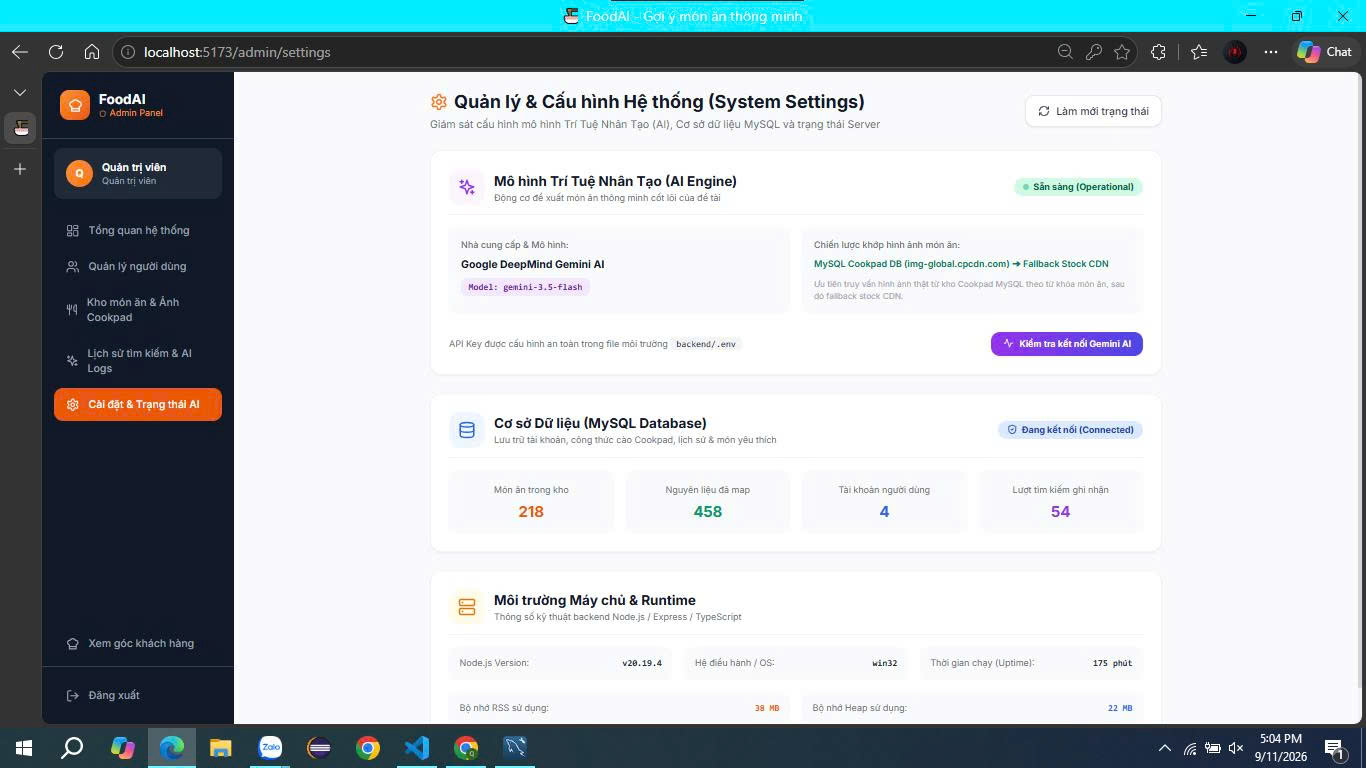
\includegraphics[width=0.96\textwidth]{figs/ui_admin_cai_dat_he_thong.jpg}
\caption{Giao diện Cấu hình Hệ thống, Giám sát Mô hình AI Gemini và CSDL MySQL.}
\label{fig:ui_admin_settings}
\end{figure}

\noindent\textbf{Mô tả:} Hình~\ref{fig:ui_admin_settings} thể hiện trang Cấu hình \& Giám sát Hệ thống, chia làm 3 khối thông tin: Trạng thái mô hình AI Gemini (kèm nút kiểm tra kết nối trực tiếp), Trạng thái cơ sở dữ liệu MySQL (số lượng bản ghi món ăn, nguyên liệu) và Thông số môi trường máy chủ Node.js (phiên bản, hệ điều hành, uptime, dung lượng RAM sử dụng).

\noindent\textbf{Diễn giải:} Trang này cung cấp công cụ chẩn đoán nhanh toàn bộ hạ tầng kỹ thuật của FoodAI. Quản trị viên có thể kiểm tra tức thì trạng thái sẵn sàng của Google Gemini API chỉ với một cú nhấp chuột, nắm bắt chính xác mức tiêu thụ bộ nhớ RAM và thời gian hoạt động liên tục của máy chủ để chủ động bảo trì hạ tầng.

\section{Kiểm thử hệ thống}

Quá trình kiểm thử được tiến hành có hệ thống trên nhiều nhóm kịch bản nghiệp vụ (Bảng~\ref{tab:kiemthu}).

\begin{table}[H]
\centering
\caption{Bảng tổng hợp các ca kiểm thử chức năng và ngoại lệ hệ thống.}
\label{tab:kiemthu}
\begin{tabularx}{\textwidth}{@{}>{\bfseries\color{daunavy}}p{1.4cm} >{\color{daumaroon}\raggedright\arraybackslash}X >{\raggedright\arraybackslash}X >{\centering\arraybackslash\color{forestgreen}\bfseries}p{2.2cm}@{}}
\toprule
\rowcolor{gray100}\bfseries\color{daunavy}Mã ca & \bfseries\color{daumaroon}Dữ liệu đầu vào & \bfseries\color{daunavy}Kết quả kỳ vọng & \bfseries\color{forestgreen}Trạng thái \\
\midrule
TC-01 & Email, mật khẩu hợp lệ & Đăng nhập thành công, cấp JWT token & Đạt (Pass) \\
TC-02 & Nguyên liệu: [thịt bò, cà chua, hành tây] & Gợi ý 4--6 món chuẩn vị bò, có dinh dưỡng & Đạt (Pass) \\
TC-03 & Nguyên liệu chay: [trứng, đậu phụ, nấm] & 100\% món không có thịt/cá, không ảo giác & Đạt (Pass) \\
TC-04 & Tắt kết nối Internet / API Key trống & Tự động Fallback sang kho Cookpad MySQL & Đạt (Pass) \\
TC-05 & User thường truy cập route \code{/admin} & Bị chặn và chuyển hướng về \code{/dashboard} & Đạt (Pass) \\
TC-06 & Nhập chuỗi rỗng / ký tự đặc biệt & Thông báo lỗi tiếng Việt thân thiện & Đạt (Pass) \\
\bottomrule
\end{tabularx}
\end{table}

\noindent\textbf{Mô tả:} Bảng~\ref{tab:kiemthu} tổng hợp kết quả thực thi 6 ca kiểm thử tiêu biểu (TC-01 đến TC-06) trên các kịch bản chức năng chính và xử lý ngoại lệ: xác thực tài khoản, gợi ý món thịt, kiểm soát món chay không ảo giác đạm lạ, cơ chế dự phòng Fallback khi mất mạng, bảo mật phân quyền đường dẫn quản trị và kiểm tra tính hợp lệ của chuỗi nhập liệu.

\noindent\textbf{Diễn giải:} Kết quả 100\% ca kiểm thử đều đạt trạng thái Đạt (Pass) chứng minh chất lượng phần mềm đạt độ tin cậy và sự hoàn thiện cao. Hệ thống hoạt động chính xác theo đúng các ràng buộc thiết kế: đáp ứng tốt yêu cầu nghiệp vụ thông thường, đồng thời tự động kích hoạt các chốt chặn phòng thủ khi gặp dữ liệu xấu, tấn công vượt quyền hoặc sự cố đứt kết nối dịch vụ AI bên ngoài.
